\documentclass{article}


% if you need to pass options to natbib, use, e.g.:
%     \PassOptionsToPackage{numbers, compress}{natbib}
% before loading neurips_2024


% ready for submission
%\usepackage{neurips_2024}


% to compile a preprint version, e.g., for submission to arXiv, add add the
% [preprint] option:
\usepackage[preprint]{neurips_2024}


% to compile a camera-ready version, add the [final] option, e.g.:
%     \usepackage[final]{neurips_2024}


% to avoid loading the natbib package, add option nonatbib:
%    \usepackage[nonatbib]{neurips_2024}

\usepackage{csquotes}
\usepackage{paralist}
\usepackage{adjustbox}
\usepackage{enumitem}
\usepackage{graphicx}
\usepackage{booktabs}
\usepackage[utf8]{inputenc} % allow utf-8 input
\usepackage[T1]{fontenc}    % use 8-bit T1 fonts
\usepackage{hyperref}       % hyperlinks
\usepackage{url}            % simple URL typesetting
\usepackage{booktabs}       % professional-quality tables
\usepackage{amsfonts}       % blackboard math symbols
\usepackage{nicefrac}       % compact symbols for 1/2, etc.
\usepackage{microtype}      % microtypography
\usepackage[dvipsnames]{xcolor}         % colors
\usepackage{tikz}
\usepackage{doi} 

\renewcommand{\subsectionautorefname}{Subsection}


\usetikzlibrary{positioning, arrows.meta,decorations.pathreplacing,calc,shapes.geometric}

\setcitestyle{numbers,square}
\bibliographystyle{abbrvnat}

%\title{LLM-enhanced Robot Swarms that Responsively Reason, Plan, and Collaborate}
\title{LLM2Swarm: Robot Swarms that Responsively Reason, Plan, and Collaborate through LLMs}


% The \author macro works with any number of authors. There are two commands
% used to separate the names and addresses of multiple authors: \And and \AND.
%
% Using \And between authors leaves it to LaTeX to determine where to break the
% lines. Using \AND forces a line break at that point. So, if LaTeX puts 3 of 4
% authors names on the first line, and the last on the second line, try using
% \AND instead of \And before the third author name.


\author{%
  Volker Strobel\\
  IRIDIA\\
  Universit\'e Libre de Bruxellles\\
  Brussels, Belgium \\
  \texttt{volker.strobel@ulb.be} \\
  \And
  Marco Dorigo\\
  IRIDIA\\
  Universit\'e Libre de Bruxellles\\
  Brussels, Belgium \\
  \texttt{mdorigo@ulb.ac.be} \\
  \AND
  Mario Fritz\\
  CISPA Helmholtz Center for Information Security\\
  St. Ingbert, Germany\\
  \texttt{fritz@cispa.de}
}



\newif\ifcmnts
\cmntstrue


\newcommand{\myparagraph}[1]{\paragraph{#1}}
\newcommand{\cmnt}[1]{\ifcmnts{\color{red}{\textbf{#1}}}\fi}
\renewcommand{\myparagraph}[1]{}

\newif\ifcomments
\commentstrue

\newcommand{\mario}[1]{\ifcomments{\color{blue}{mario: #1}}\fi}
\newcommand{\volker}[1]{\ifcomments{\color{Green}{volker: #1}}\fi}


% I added this command to hide Mario's comments that I already addressed
\newif\ifshowresolved
\showresolvedfalse

\newcommand{\rmario}[1]{\ifshowresolved{\color{blue}{mario: #1}}\fi}
\newcommand{\rvolker}[1]{\ifshowresolved{\color{Green}{volker: #1}}\fi}

\begin{document}
\maketitle

\iffalse
\section*{TODOs}

\begin{itemize}
%\item  Autonomy: a pretrained LLM incoprorates prior background knowledge and common sense about situations that the swarm may not have encountered before (see also zero shot learning and out-of-distribution detection) - therefore, it can prevent to execute stupid actions and adapt a plan online; in particular, it may also incoprorate moral values of humans and therefore favor 'morally good' actions
 %\item We could develop a taxonomy about opportunities and challenges -- and highlight existing problems  
\item Swarm controller synthesis gym/benchmark (note: this could be mentioned in the first paper and elaborated in a second paper; however, we should be fast then to publish the second paper!)

\end{itemize}
\fi

\begin{abstract}
\rmario{concerning title "LLM-enhanced" sounds very incremental - as if we won't expect any qualitative improvements or disruptive changes. maybe "LLM-enabled" is better? I'm trying different rephrasings I'd also brand this as "LLM2Swarm"} \rvolker{LLM2Swarm sounds good to me. Also LLM-enabled is fine for me  -- it first sounded a bit strange but then I realized that it is very similar to other uses, like in `Bluetooth-enabled device'. An alternative to LLM-enabled could be LLM-integrated as `integration' is the word we use most-often in the paper.}

Robot swarms are composed of many simple robots that communicate and collaborate to fulfill complex tasks. Robot controllers usually need to be specified by experts on a case-by-case basis via programming code. This process is time-consuming, prone to errors, and unable to take into account all situations that may be encountered during deployment. On the other hand, recent Large Language Models (LLMs) have demonstrated reasoning and planning capabilities, introduced new ways to interact with and program machines, and incorporate both domain-specific and commonsense knowledge. Hence, we propose to address the aforementioned challenges by integrating LLMs with robot swarms and show the potential in proofs of concept (showcases). For this integration, we explore two approaches. The first approach is `indirect integration,' where LLMs are used to synthesize and validate the robot controllers. This approach may reduce development time and human error before deployment. Moreover, during deployment, it could be used for on-the-fly creation of new robot behaviors. The second approach is `direct integration,' where each robot locally executes a separate LLM instance during deployment for robot-robot collaboration and human-swarm interaction. These local LLM instances enable each robot to reason, plan, and collaborate using natural language, as demonstrated in our showcases where the robots are able to detect a variety of anomalies, without prior information about the nature of these anomalies. To enable further research on our mainly conceptual contribution, we release the software and videos for our LLM2Swarm system: \url{https://github.com/Pold87/LLM2Swarm}.
\rmario{I'm still not sure about "indirect" vs "direct". could it also be "pre-mission" and "in-mission"? I'll read on and come back to this.} \rvolker{I am not sure either and am open for suggestions. Previously, I had `offline' and `online', with the meaning of `pre-mission' and `in-mission'. However, I think the real difference lies in whether or not you use the LLM output directly or via the indirect route of controller generation/synthesis.}\rmario{yes - maybe then it's more "synthesis-based" vs "interactive"; well - maybe "direct" vs "indirect" integration is not so bad actually}
\end{abstract}

\section{Introduction}

\rmario{high level comment: i like the reason, plan, collaborate slogan .... but it should also reappear somewhere in the submission. E.g. text or structuring elements - like headings}\rvolker{I added the slogan to Opportunities.}

Robot swarms consist of many simple robots that accomplish complex tasks by collaborating with each other~\cite{DorTheTri2020:scirobotics,Ham2018:book}. They are characterized by the absence of a central control unit, which makes them more scalable and flexible than other multi-robot systems. Thanks to their decentralized control and redundancy, robot swarms can potentially continue functioning even if individual robots fail~\cite{WinNem2006:mic}. These features could make robot swarms ideal for applications where fast reactions to unforeseen events are required, such as environmental monitoring and disaster response~\cite{DorTheTri2021:pieee,YanBelDup-etal2018:scirobotics}.

\rmario{the statement "often simple robots" is a key requirement/point in your argumentation - and I'm afraid it might be overlooked. you need to make it more prominent and not optional (as in "often") - I think. You need it in multiple places below: (1) clearly delimit your work from prior work on general robots with LLMs (2) motivate the control synthesis for responsiveness.} \rvolker{I was a bit afraid of using 'simple' because people in swarm robotics then might think of Kilobots, which have a 8MHz processor. and will never be able to run LLMs... but I agree, it is one of the main selling points and I added 'simple' to the first sentence and removed this sentence as it was redundant.}

In robot swarms, communication and interaction protocols between robots usually need to be specified by experts on a case-by-case basis via programming code~\cite{Kuc2023:frontiers}: Given a specific task, a human designer needs to develop and implement the corresponding program logic. The process of writing such code is often time-consuming and prone to errors. Even though there are attempts to automate this process~\cite{FraBraBru-etal2014:si,GarBir2024:icra,TriTucAmpDor2014:evorobotics,TolGamPaul-etal2020:roblearning,FinMetMos2022:cav}, these attempts usually still require expert knowledge at design time  and the controllers cannot react to unforeseen events at deployment time.

Recent advances in Large Language Models (LLMs) have led to new possibilities and proposals for the integration of AI into different technologies, such as virtual assistants and search engines~\cite{GreAbdMis-etal2023:aisec}. In particular, there have also been proposals to integrate LLMs into multi-robot systems~\cite{CheArkZha-etal2024:icra,ManJaiSon2023:icra}. With this paper, we propose to integrate LLMs into a specific kind of multi-robot system: robot swarms.

We provide the first systematic exploration of the potential of LLM-enabled robot swarms (we call our system LLM2Swarm). We demonstrate the resulting opportunities in a series of proofs of concept (showcases), implemented in the ARGoS robot swarm simulator~\cite{PinTriOGr-etal2012:si}, and preliminary hardware tests using a Raspberry Pi~5. For this exploration, we propose two primary approaches of integrating LLMs into robot swarms. 

The first approach is ``indirect integration,'' where LLMs are used to synthesize and validate the robot controllers (before and/or during deployment). This approach may save development time for the designer by automating parts of the design process. In addition, it could dramatically simplify the process of writing controllers, as no programming knowledge is necessary. The approach ensures that robot swarms \emph{responsively} react, as they execute their classical (synthesized) control software, instead of waiting for LLM-generated responses.

The second approach for integrating LLMs into robot swarms is ``direct integration,'' where each robot locally executes a separate LLM instance during deployment. With this online integration, the local LLM instances enable each robot to reason, plan, and collaborate using natural language. With these new and improved capabilities, we aim to enhance robot swarms' adaptivity, efficiency, and intelligence, making them more capable of handling complex tasks in unpredictable environments, both for robot-robot collaboration and human-swarm interaction.

%The decision on when to use which approach depends on the trade-offs involved. Indirect use may be more suitable for applications where responsive reactions and simplicity are important. Direct use offers greater flexibility and intelligence at the cost of higher computational requirements and complexity. Choosing the correct design is crucial for the successful deployment of LLM-enhanced robot swarms in real-world scenarios.

In summary, our contributions are as follows:%
\begin{enumerate}
    \item We introduce LLM2Swarm for integrating LLMs into robot swarms and explore the resulting opportunities and challenges.
    \item We provide (video) showcases for controller synthesis, robot-robot collaboration, and human-swarm interaction in simulation.
    \item We release our LLM2Swarm setup as open-source software. Videos and code can be downloaded at \url{https://github.com/Pold87/LLM2Swarm}.
\end{enumerate}

\begin{figure}
    \centering
    \includegraphics[width=0.95\textwidth]{img/temporal_flow_nonbold-2.drawio-2.pdf}
    \caption{\textbf{Overview of LLM2Swarm -- LLM-enabled robot swarms}. LLM2Swarm involves four key system components: humans, LLMs, controllers, and platforms.
    \emph{Before mission start}: a human designer uses both manual design and LLM2Swarm's controller synthesis module (which prompts a powerful LLM) to generate a robot controller. This controller is executed in simulation, and uses one lightweight LLM per robot to simulate on-device execution of LLM2Swarm's direct integration module. \emph{After mission start}: a human operator interacts with the real robots' lightweight on-device LLMs to instruct the swarm and to receive information about the swarm state. These LLMs also interact with other robots' controllers in order to reason, plan, and collaborate. In addition, the lightweight LLMs can synthesize new robot controllers on-the-fly during the mission.}
    \label{fig:temporal-flow-interactions}
\end{figure}


\section{Related work}
\label{sec:related-work}

Our work is related to three topics: controller synthesis, LLMs as agents, and LLMs in robotics. In the following, we briefly present related work from these fields and highlight how our vision differs.

\textbf{Controller synthesis.}
There are several related works on controller synthesis, both from the field of swarm robotics (e.g., AutoMoDe~\cite{FraBraBru-etal2014:si,GarBir2024:icra}, evolutionary approaches~\cite{TriTucAmpDor2014:evorobotics}, neural network controllers~\cite{TolGamPaul-etal2020:roblearning}) and from more theoretical fields, such as computer aided verification~\cite{FinMetMos2022:cav}. LLMs have also already been used for the controller synthesis of single robots~\cite{VemBonBucKap2024:techrep}. However, these approaches still rely on expert knowledge (e.g., formal specification languages) during design time, cannot flexibly react to unforeseen situations during deployment, or do not support multiple agents or robots.


\textbf{LLMs in multi-agent systems.}
LLMs are increasingly being integrated into other systems to enhance their capabilities (e.g., as part of search engines)~\cite{GreAbdMis-etal2023:aisec}.
In the recent past, there has been an increasing interest in letting \emph{multiple} LLMs interact and discuss~\cite{AbdGomSiv-etal2024:arxiv,ChuGoyHar-etal2023:arxiv}.
An overview of the integration of LLMs into multi-agent systems for various tasks has been given by Guo et al.~\cite{GuoCheWan-etal2024:arxiv}. In contrast to these works, our target platforms are physical robots. The previous works did not take into account how to synthesize robot controllers, how to deal with mobility, sensor information, and actuators, and how to map sensors and actuators to LLM inputs and responses.


\textbf{LLMs in robotics.}
Integrating LLMs into other systems has also led to several new applications in robotics~\cite{KimKimCho-etal2024:intellservicerobotics}, for example for task planning~\cite{DinZhaAmi-etal2023:autorob}, centralized motion planning~\cite{JiaPatKhu-etal2023:neurips}, and human-robot interaction~\cite{VemBonBucKap2024:techrep}.
%To the best of our knowledge, there is no existing research that integrates LLMs into robot swarms.
%Yet, there have been proposals to integrate LLMs into multi-agent systems and into some robotic systems. %We discuss these research lines below.
%Language models can be classified into small language models (SLMs) and large language models (LLMs)\cite{TODO}. 
%The difference is made based on the number of parameters these models have: 
%In general, SLMs are less powerful and task-specific, whereas pre-trained LLMs are general-purpose models   suitable for any task (i.e., they are task-agnostic).
%This  rendering them potentially suitable for any swarm robotics task.
%For example, ROSGPT is a package that provides an interface between the software ROS2 and ChatGPT in order to facilitate human-robot interaction.  
%There is also already some related work on the combination of LLMs and multiple robots.
As our target platforms are robot swarms, in the following, we are considering works that use a separate LLM instance for each embodied agent. %For this, we identified three notable papers.
%In contrast to the above-mentioned multi-robot papers that used centralized LLMs, our vision is to decentralize the framework and have separate LLM instance for each robot.
%This has been proposed by \citeauthor{DasKaeMar-etal2023:arxiv}~\cite{DasKaeMar-etal2023:arxiv}.  
%
\citeauthor{CheArkZha-etal2024:icra}~\cite{CheArkZha-etal2024:icra} perform motion planning (e.g., to move a box to a target), with up to 32~simulated robots (in 2D grid environments and using robotic arms).
%In contrast to our work, they do not consider mobile robots.
%global communication and do not perform any hardware experiments or demonstrations.
\citeauthor{ManJaiSon2023:icra}~\cite{ManJaiSon2023:icra} perform motion planning (of robotic arms) with up to three robots.
%However, their setup is centralized as the robots rely on a single external cloud-based LLM.
%In addition, they only study systems composed of three robots and do not use mobile robots.
\citeauthor{ZhaDuSha-etal2024:iclr}~\cite{ZhaDuSha-etal2024:iclr} study how two virtual humans can communicate via LLMs. 
These research efforts, however, have one or more of the following limitations: a low number of robots/agents, lack of decentralization, no consideration of mobile robots with physics-based dynamics, no consideration of typical swarm robotics tasks, or no consideration of hardware limitations; therefore, their applicability to swarm robotics is limited.
%However, their study is rather different from our proposal, as they are dealing with a very low number of humanoid agents (two agents) and are therefore not addressing any tasks which typically are envisioned to be performed by robots. 

% \subsubsection{TODO}

% Papers to check (based on Guo et al. - Large Language Model based Multi-Agents: A Survey of Progress and Challenges):

% \begin{itemize}
%     \item [Dasgupta et al., 2023] Ishita Dasgupta, Christine Kaeser-Chen, Kenneth Marino, Arun Ahuja, Sheila Babayan, Felix Hill, and Rob Fergus. Collaborating with language models for embodied reasoning. arXiv preprint arXiv:2302.00763, 2023
% \item [Mandi et al., 2023] Zhao Mandi, Shreeya Jain, and Shuran Song. Roco: Dialectic multi-robot collaboration with large language models. arXiv preprint arXiv:2307.04738, 2023.
% \item [Zhang et al., 2023c] Hongxin Zhang, Weihua Du, Jiaming Shan, Qinhong Zhou, Yilun Du, Joshua B Tenenbaum, Tianmin Shu, and Chuang Gan. Building cooperative embodied agents modularly with large language models. arXiv preprint arXiv:2307.02485, 2023.
% \item [Chen et al., 2023d] Yongchao Chen, Jacob Arkin, Yang Zhang, Nicholas Roy, and Chuchu Fan. Scalable multi-robot collaboration with large language models: Centralized or decentralized systems? arXiv preprint arXiv:2309.15943, 2023.
% \item [Yu et al., 2023] Bangguo Yu, Hamidreza Kasaei, and Ming Cao. Co-navgpt: Multi-robot cooperative visual semantic navigation using large language models, 2023.
% \item [Chen et al., 2023b] Huaben Chen, Wenkang Ji, Lufeng Xu, and Shiyu Zhao. Multi-agent consensus seeking via large language models. arXiv preprint arXiv:2310.20151, 2023
% \end{itemize}

\section{LLM-enabled robot swarms: LLM2Swarm}


\rmario{there is a section missing right before "Opportunities" that explains our approach to integrating LLMs in swarms. this needs to settle terminology and use figure 1 to describe the overall landscape. I moved a bit of text around (from caption to here and start of opportunities) ... but there needs to be a bit more describing our main idea and the topologie/structure. this is one of our core contributions! this should not be entangled with opportunities and challenges. before - the main method/approach/structure was described in the captions - this is not good.}

To give an overview of how our LLM2Swarm system yields LLM-enabled robot swarms, we illustrate the proposed temporal flow and interactions in \autoref{fig:temporal-flow-interactions}.
%We believe that LLMs have the potential to largely enhance the capabilities of robot swarms.
LLM2Swarm provides two main modules: an \emph{indirect integration module} for automating controller design (both before and during deployment) and a \emph{direct integration module} for enhancing robots' reasoning, planning, and collaboration capabilities during deployment.
%These enhancements might lead to an overall greater autonomy and intelligence of robot swarms. % and, thanks to the transparency provided by the natural language interactions, could also lead to a greater acceptance and trust by humans.

\rvolker{TODO: Check if this can be included somewhere: : the mission start marks a crucial event in the life cycle of LLM-enabled robot swarms: at this point and after, the LLMs that reason, plan, and collaborate need to be executed on-board of real robots.}


%\subsection{Temporal flow of interactions between humans, LLMs, controllers, and platform} Before the mission start, a human designer generates robot controllers, using powerful LLMs and manual design. 

%In addition, lightweight LLMs, identical to those employed during deployment, are used in simulation to test their capabilities and the resulting robot behavior. 



\subsection{Indirect Integration}

We propose to use LLMs `indirectly' for controller synthesis, i.e., automated creation of code before or during deployment. For this indirect integration, LLM2Swarm provides a module (see \autoref{fig:controller-generation}) that translates a description of a robot controller in natural language to an actual robot controller.
%As illustrated in \autoref{fig:controller-generation}, the `indirect use' of LLMs for generating and synthesizing controllers involves the user who specifies the required functionality.
Before the mission start, a human designer generates a robot controller draft using manual design. Parts of these controllers can be synthesized by LLM2Swarm, using a powerful LLM (LLM2Swarm supports any model provided by OpenAI's API or by Ollama for local execution).
%\cmnt{TODO: add here what happens after the mission start: the code is synthesized using the on-board devices -- or the human sends updates using LLMs that were executed outside of the swarm.}
Also during deployment, this LLM2Swarm module can lead to increased autonomy of a robot swarm---as missing controller parts can be synthesized on the fly by on-board LLMs.
%
Based on our experiments, we propose the following three-step process to automate controller synthesis:%
\paragraph{Step~1 -- Syntax validation.} The first validation is to check whether a synthesized controller contains syntactically correct and executable code.
%During our experimentation, we experienced that the first versions of such a generated controller often contain errors (for example, because it contained function skeletons rather than full specifications). For this reason, it is often necessary to run multiple iterations of controller generation, until the errors are resolved. %\footnote{In our experiments, the synthesized code often contained placeholder functions, with the instruction for the user to fill them in, even though we explicitly mentioned that we desire a plug-and-play solution. In addition, some code resulted in type errors in Python (e.g., when the synthesized controller used \texttt{float} as data type when \texttt{Vector2D} was expected).} 
Consequently, a syntax validator is essential to prevent the execution of erroneous code, which could lead to disastrous outcomes (e.g., erroneous code controlling a drone could result in crashes and severe hardware damage).

\paragraph{Step~2 -- Logic validation.}Validating whether the generated code performs the intended task as expected is crucial but challenging, as there is not always a clear ground truth. If the code is synthesized before deployment, its resulting behavior can be analyzed and improved using LLM2Swarm---either by human feedback or in the future by the video analysis capabilities of LLMs 
%After these iterations, similar iterations could be performed for logic validation and security checking, until the final controller is generated.
%While we have not yet implemented logic validation and security checking 
(although the current video analysis capabilities are limited\footnote{Even though OpenAI's API does not yet support video analysis, in a preliminary experiment, %\rmario{"briefly" does not have any meaning in a scientific paper ... and you want to avoid any notion of adhoc or half-done impressions. . you can call it "initial" or "preliminary"  experiments}\rvolker{Makes sense - changed to preliminary experiment.}
we tested ChatGPT-4o's video analysis capabilities by uploading a video of \emph{random-walk} behavior in an ARGoS simulation and asking whether the swarm demonstrated successful \emph{flocking} behavior. The LLM's analysis was unsatisfactory, as it incorrectly concluded that the behavior was successful flocking behavior.}, we believe that future developments will improve this capability). During deployment, however, such verification is usually not possible---in addition, simulations cannot account for all possible real-world scenarios. Alternatives for evaluating a controller during deployment could be reinforcement learning to compare different controllers~\cite{BlaAkh2023:cognitiverobotics} or probabilistic model checking based on mathematical analysis~\cite{KonDixFis2021:ras}.
%For example, in a foraging scenario, the robots could evaluate which controller would lead to the most gathered resources. %Reinforcement learning might, however, be susceptible to the problems of goal misgeneralization and goal misspecification~\cite{ShaVarKum2022:arxiv}.
%Another alternative could be .
%This approach allows the formulation of detailed performance metrics and can help in identifying potential anomalies before actual deployment.

\paragraph{Step~3 -- Security checking.} It is important to verify whether the LLM-synthesized controller contains security issues or potentially malicious parts (e.g., the controller could contain logic to sabotage other robots). Identifying security issues can be based on the \emph{Common Weakness Enumeration} (CWE), a catalog that lists known exploits in programming languages and hardware components\footnote{\url{https://cwe.mitre.org/}, accessed September 20, 2024}. In addition, there are model checkers and LLMs fine-tuned to the task of identifying weaknesses that are part of the CWE. LLM2Swarm enables preliminary security checking through an LLM prompt with the request of identifying malicious parts and other weaknesses in a synthesized controller.

\begin{figure}
    \centering
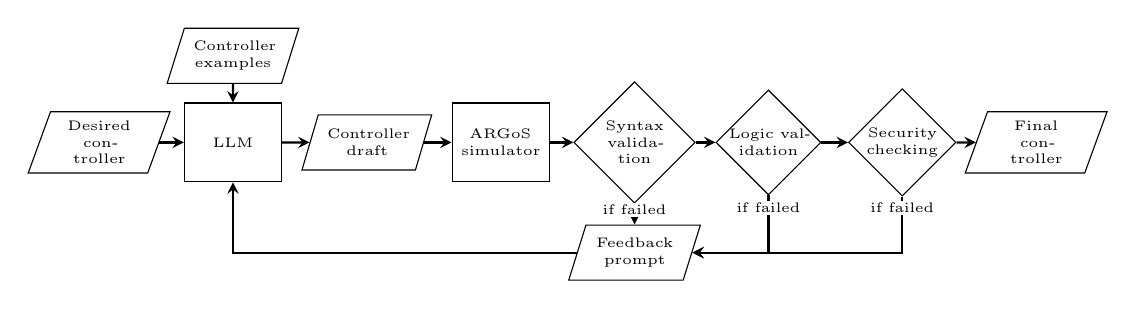
\begin{tikzpicture}[node distance=1.7cm,font=\tiny]
    \tikzstyle{startstop} = [rectangle, rounded corners, 
minimum width=1cm, 
minimum height=1cm,
text centered, 
text width=1cm,
draw=black]

\tikzstyle{io} = [trapezium, 
trapezium stretches=true, % A later addition
trapezium left angle=70, 
trapezium right angle=110, 
minimum width=1.0cm, 
minimum height=0.7cm, text centered, 
text width=1.0cm,
draw=black]

\tikzstyle{process} = [rectangle, 
minimum width=1cm, 
minimum height=1cm, 
text centered, 
text width=1cm, 
draw=black]

\tikzstyle{decision} = [diamond, 
minimum width=0.7cm, 
minimum height=1cm, 
text centered, 
text width=1.0cm,
inner sep=0pt,
draw=black]
\tikzstyle{arrow} = [thick,->,>=stealth]


\node (in1) [io] {Desired controller};
\node (llm) [process, right of=in1, xshift=0cm] {LLM};
\node (examples) [io, above of=llm, yshift=-0.6cm] {Controller examples};
\node (controllerdraft) [io, right of=llm] {Controller draft};
\node (argos) [process, right of=controllerdraft] {ARGoS\\simulator};
\node (syntaxvalidation) [decision, right of=argos] {Syntax validation};
\node (logicvalidation) [decision, right of=syntaxvalidation] {Logic validation};
\node (securitychecking) [decision, right of=logicvalidation] {Security checking};
\node (finalcontroller) [io, right of=securitychecking] {Final controller};
\node (feedback) [io, below of=syntaxvalidation,yshift=0.3cm] {Feedback prompt};

% \node (pro2a) [process, above of=dec1, yshift=-0.5cm] {Process 2a
% text text text text
% text text text 
% text text text};

% \node (pro2b) [process, right of=dec1, xshift=2cm] {Process 2b};
% \node (out1) [io, below of=pro2a] {Output};
% \node (stop) [startstop, below of=out1] {Stop};

\draw [arrow] (in1) -- (llm);
\draw [arrow] (examples) -- (llm);
\draw [arrow] (llm) -- (controllerdraft);
\draw [arrow] (controllerdraft) -- (argos);
\draw [arrow] (argos) -- (syntaxvalidation);
\draw [arrow] (syntaxvalidation) -- (logicvalidation);
\draw [arrow] (logicvalidation) -- (securitychecking);
\draw [arrow] (securitychecking) -- (finalcontroller);
\draw [arrow] (syntaxvalidation) -- node[yshift=0.05cm,fill=white,inner sep=0.8pt] {if failed} (feedback);
\draw [arrow] (logicvalidation) |- node[yshift=0.57cm,fill=white,inner sep=0.8pt] {if failed}(feedback);
\draw [arrow] (securitychecking) |- node[yshift=0.57cm,fill=white,inner sep=0.8pt] {if failed} (feedback);
\draw [arrow] (feedback) -| (llm);


\end{tikzpicture}
    \caption{\textbf{Flow of LLM2Swarm's controller synthesis module}. Using LLM2Swarm's controller synthesis module, a user begins by specifying the desired controller in natural language. This specification, together with controller examples, is used as part of an LLM prompt to synthesize a robot controller. The synthesized controller draft is then executed directly in the ARGoS simulator. If ARGoS detects any syntax errors, the errors are reported back to the LLM, with the request to resolve them. If no syntax errors are found, the user can proceed to validate the controller logic: if the robot behavior is not as expected, the user provides information about both the robots' expected behavior and actual behavior to the LLM with the request to improve the controller. Once the controller logic is validated, the user can ask the LLM to check for any security vulnerabilities. After all validation steps are completed, the final controller, specified in programming code, is ready for deployment.}
    \label{fig:controller-generation}
\end{figure}

\subsection{Direct Integration}

For directly integrating LLMs into robot swarms, we propose to execute one LLM per robot, locally on each robot's hardware (see \autoref{fig:system-interaction}), which requires lightweight LLMs. Currently, LLM2Swarm \emph{simulates} local execution: In our showcases, each robot is connected to a separate \emph{external} LLM, allowing us to run LLMs of any capacity and thus simulate today what we anticipate for the future.
For direct integration, the LLMs' prompts are fed with sensor information (including messages received from other robots), and the outputs of the LLMs are mapped to robot actions. 
%The mission start marks crucial event in the life cycle of LLM-enabled robot swarms: at this point and after, the LLMs that reason, plan, and collaborate need to be executed on-board of real robots
During deployment, a human operator may interact with these on-board LLMs to supervise the mission.

\begin{figure}
    \centering
    \includegraphics[width=0.85\linewidth]{img/system_int.pdf}
    \caption{\textbf{System interactions for LLM2Swarm's direct integration module.} Using LLM2Swarm's direct integration module, a robot's controller is composed of two parts: a classical controller and an on-device LLM. As in traditional approaches, the classical controller manages the robot's actuators and sensors. However, unlike traditional approaches, the controller also creates prompts for the on-device LLM and uses the responses to guide the robot's actions. This on-device LLM also enables a robot to interact with other robots or a human operator by using natural language. As a result, such LLM-enabled robots can reason, plan, and collaborate thanks to the capabilities of their on-device LLMs.}
    \label{fig:system-interaction}
\end{figure}


 
\subsection{Experiment setup}
\label{sec:experiment-setup}

%In this section, we describe the setup for our experiments, which are, depending on the showcase, either implemented in the ARGoS robot swarm simulator using Pi-puck robots or using a physical Raspberry Pi~5. These showcases are intended to highlight both current capabilities and anticipated future advancements in robot swarms.


%\subsubsection{Simulation environment}
In our showcases, we simulate Pi-puck robots using the widely-used robot swarm simulator ARGoS~\cite{PinTriOGr-etal2012:si} (version 3.0.0-beta56) on a personal computer (OS: Ubuntu 22.04.4 LTS, CPU: Intel Core i7-8550U\,@\,1.80~GHz, RAM: 16~GB, GPU: Intel UHD Graphics 620). Although ARGoS controllers are usually written in C\texttt{++}, we use the ARGoS-Python interface~\cite{HasParPacStr2024:software} (version v1.0.0), enabling us to easily connect each simulated robot to an LLM instance (we use GPT-4o). %We also use GPT-4o for the purposes of controller design and video analysis.
%In the experiments, in which the robots execute local LLMs, we use Ollama and select Microsoft's Phi-3 LLM. 

%\subsubsection{Hardware experiments}
%The hardware experiments are executed on the single-board processor Raspberry Pi 5, using Ollama and a variety of LLM instances. 

\section{Opportunities}
\label{sec:opportunities}

\rmario{short outline of the opportunities section}

In this section, we explore the opportunities that are enabled by LLM2Swarm: automated controller synthesis, enhanced robot-robot collaboration, and more intuitive human-swarm interaction.
%Overall, we believe that LLM2Swarm can enhance robot swarms' adaptability, efficiency, and intelligence, making them more capable of handling complex tasks in unpredictable environments and of establishing new modes for human-swarm interaction.  

\subsection{Automated controller synthesis}
\label{sec:automated-controller-generation}

Synthesizing controllers maintains the \emph{responsiveness} of a robot swarm, as this can be done before deployment or during a low-activity phase during deployment. Overall, this automated controller synthesis can lead to faster development times, the specification of controllers by non-experts, and on-the-fly adaptation of robot controllers during deployment.

For creating controllers by LLMs, different design choices need to be made. It needs to be decided whether the LLM should synthesize the complete controller or only specific parts (e.g., only the movement logic). Another design choice is whether the controller (parts) should be written by an LLM before or rather during deployment. These design choices balance the trade-off between autonomy and controllability (see also \autoref{sec:controllability}).


% In order to showcase the potential of LLMs for generating controllers, we have used the following prompt:%
% \begin{quote}
% Create a spinning algorithm. The robots should spin in circles for 100 time steps. Then stop for 25 time steps, then spin again for 100 time steps. And so on.
% \end{quote}




\subsection{Robot-robot collaboration and human-swarm interaction}
\rmario{make sure that you always describe it in the swarm context}
\rmario{this subsection was a huge chunk of text. this is not easy for the reader. I've tried to give some more structure with the "paragraph" tags. in general, paragraphs should be shorter.}


%In real-world deployments, robot swarms may often encounter unexpected situations.

\paragraph{Robot-robot collaboration and adaptivity in swarms.}

We believe that LLM2Swarm % enables the robots to become intelligent agents capable of reasoning, planning, and collaborating, as these capabilities are built into LLMs. integration of LLMs into robot swarms
can largely improve robot-robot collaboration. First, enhancing robots with LLMs expands their ability to \emph{reason}. %Another critical advantage of this approach is that in contrast to classical robot controllers
Pre-trained LLMs incorporate general knowledge about the world and context-aware reasoning, which they can use to react to unanticipated challenges, incorporating moral values and favoring ethical actions---potentially considering how humans would react in similar situations.% (see our showcase in \autoref{fig:robot-robot-interaction}).
%For example, a swarm tasked with monitoring crop development could suddenly spot an injured person. Classical approaches, which rely on hard-coded controllers or a limited set of pre-specified behaviors, cannot handle such situations effectively.
%In contrast, pre-trained general-purpose LLMs within robot swarms could better handle these scenarios as these models, having incorporated background knowledge from diverse sources, can generate appropriate responses, 


Second, LLM2Swarm provides robots with advanced \emph{planning} capabilities. Pre-trained LLMs can generate collective plans, involving the allocation of different robots to different tasks and the ability to adapt plans in real-time (for example, to adapt a path planning procedure when unanticipated situations occur). LLMs are also able to analyze the history of interactions and decide on the best next collective action based on this.
%This can for example be used to execute a sequence of actions in the correct order.

Finally, LLM2Swarm enables robots to \emph{collaborate} using natural language, enabling more sophisticated interactions among robots and between robots and humans than classical controllers. As the interactions are expressed in natural language, they can also be easily understood by humans, making the interactions more transparent.
%, facilitating debugging, data analysis, and data forensics.
This also enhances trustworthiness and improves accountability, as human operators can audit the decisions and actions taken by the robot swarm. Overall LLM2Swarm can potentially enhance a robot swarm's effectiveness, autonomy, resilience, and security, in particular in complex, unpredictable (and unknown) environments, such as search-and-rescue missions where fast decision-making is critical. \rmario{there are also autonomy, resiliance, and security aspects (e.g. thinking of a potential military context)}\rvolker{Added autonomy and resilience above.}
%\cmnt{However, I did not know how/where to mention security.} 
%In addition, if robots use LLMs to communicate and coordinate with each other, the messages sent between robots can be easily understood by humans as they are specified in natural language; this improved transparency and facilitates data analysis and data forensics.


% \subsubsection{Robot-robot interaction}

% In order to showcase the LLM's capability to automatically detect anomalies and out-of-distribution behavior, we added the following text to the prompt:

% In another experiment, we disabled the wheels of the robots but kept the prompt unchanged. Also in this case, one of the LLMs recognized the anomaly:%


\paragraph{Human-swarm interaction.}

How to interact and collaborate as a human with a robot swarm in an effective manner while minimizing the cognitive load is an open research question~\cite{PaaCofBelStO2022:roman,PodOGrMat-etal2016:si}. We believe that LLM2Swarm could play an important role in advancing the field of human-robot and human-swarm interaction. %, thanks to the natural language processing (NLP) capabilities of LLMs. %In addition, the integration LLMs into robots facilitates and enhances human-swarm interaction.
%For example
%During deployment, a human could instruct the robot swarm using natural language or ask for information from the swarm. The LLM would translate this request into a format understood by each robot or information from the swarm into a human-readable output.
For example, a human operator could communicate with the LLMs of robot swarms through chat interfaces or voice commands, using natural language. This could be done with the goal of retrieving information about the collective state of the swarm~\cite{BroGooJunKer2016:humrobotinteract} or of sending commands. The LLMs may be able to understand the human commands \emph{within their context} (e.g., based on previous interactions, the current task that the swarm performs, or related to an object the swarm has just identified)---or ask back clarifying questions to the human operator. Moreover, in disaster response such as search-and-rescue operations, an LLM could interact with the victims using natural language (e.g., to inquire about the condition of the victims) and clarify the intentions and possible actions of the swarm (e.g., provide first aid or transport the victims to the hospital).


\section{Challenges}
\label{sec:challenges}

%Based on the showcases of the previous section,
We have identified the following main challenges for integrating LLMs into robot swarms: overcoming hardware limitations, ensuring scalability, addressing partitioning, and maintaining controllability. In the following sections, we describe each of these challenges in more detail.

\subsection{Hardware limitations}

To guarantee the autonomy of a robot swarm, the LLMs should be executed \emph{locally} on each robot's hardware, as external infrastructure might not always be accessible during deployment (e.g., in underwater operations, underground mining, or space exploration) and could result in communication bottlenecks. Additionally, this ensures that data remains local, thereby protecting privacy in compliance with regulations like the GDPR. However, this local execution is difficult, as robots in swarms are typically assumed to have limited hardware capacities, even though recent hardware developments are starting to relax this assumption~\cite{JonStudHauWin2018:frontiers}.

Scaling down hardware requirements and enabling on-board execution of LLMs on edge devices is a very active area of research; several approaches (e.g., finetuning~\cite{HowRud2018:acl}, quantization~\cite{DetLewBelZet2022:neurips,LinTanTan-etal2024:mls,LiuYuaJin-etal2024:icml}, pruning~\cite{FraAli2023:icml,MaFaWa2023:neurips}, distillation~\cite{HinVinDea2015:neurips}, and flash attention~\cite{DaoFuEr2022:neurips}) have been proposed for this.
%One popular such approach is \emph{finetuning}, which uses a larger and more computationally-intensive LLM to finetune a smaller more lightweight LLM. %Without such finetuning, the smaller LLM would not be capable of performing the required task; however, after fine-tuning it can be adapted to the given task. A downside of finetuning is that the LLM is less flexible during the deployment as it has been specialized for a particular task. 
%Another popular approach for executing LLMs on hardware with limited capacities is \emph{quantization}. Using quantization, the LLM model weights are represented with lower precision data types (e.g., using 8-bit integer values instead of a 32-bit float values).
In general, these approaches are able to reduce the storage and memory requirements of LLMs, at the expense of lower accuracy and flexibility. 
We anticipate that both ongoing developments in hardware miniaturization (e.g., of microprocessors and GPUs) and the aforementioned software advancements will soon enable the execution of powerful LLMs on robots in swarms.

%\cmnt{I added this. Not sure if it is good.}
In a preliminary test, we executed TinyLlama via Ollama on a Raspberry Pi~5---a small-scale single board processor suitable for swarm robotics hardware. Executing example prompts from our showcase in \autoref{sec:showcases-robot-robot-collaboration}, we obtained generation speeds between 10 and 12 tokens per second, indicating promising performance for robot-to-robot-collaboration and human-swarm interaction.

%Even though we believe that the trend of miniaturization will continue, there is still a need for approaches that reduce the hardware requirements in order to enable the efficient execution of LLMs on hardware typically available on robots in swarm.  

%In summary, addressing the hardware limitation problem is crucial for enabling the successful deployment of LLMs on robots. Future research should test the existing approaches in order to evaluate their suitability for typical swarm robotics platforms, followed by a refinement of the approaches and the development of new approaches tailored to swarm robotics.    

\subsection{Scalability}

Addressing scalability---that is, maintaining system stability when the number of robots increases---is another critical challenge when deploying LLM-integrated robot swarms.%Scalability in LLM-integrated robot swarms is impacted by token limits and processing time requirements of LLMs:
The higher the number of robots, the higher the number of potential inter-robot interactions. As the results of such inter-robot interactions may be necessary for a prompt, a higher number of them can make the prompt very complex, potentially exceeding token limits or leading to prolonged response times. Additionally, LLMs can favor verbosity over conciseness~\cite{SaiWacWatAki2023:neuripsworkshop}, which can negatively impact the efficiency of LLM-enabled robot swarms in terms of computational load and communication overhead.
%The potential exponential increase in token requirements could be mitigated if the local communication capabilities of robots in swarms are exploited: those communication limitations restrict the possible direct interactions with other robots to a robot's close neighborhood.
The potential exponential increase in token requirements could be reduced by restricting the robots' communication radius, in order to limit the number of messages exchanged with nearby robots.

%Scalability can be further hindered, as most LLMs do not have a memory; they rather require again the history of all relevant interactions, so scaling the number of robots scales up the context token requirements and runtime of the LLM. This necessitates new strategies for summarizing the history of interactions. 

\subsection{Partitioning}

Robot swarms may get partitioned into disconnected subswarms, halting the information flow between them. During such partitioning, the conversations in the subswarms might largely differ and different subswarms might not understand each other when they eventually reconnect. The partitioning problem could be partially reduced if the LLM itself controlled the robot actuators (e.g., rotors of drones) in a way that decreases the risk of partitioning. In addition, the LLMs could analyze the communication patterns and propose to execute a control logic dedicated to finding other subswarms if there is the risk of prolonged disconnections.

Still, new procedures are needed that enable both the autonomy of subswarms and the reconciliation of subswarm conversations. A possibility is to use blockchain technology for obtaining consistent states, as demonstrated in previous research~\cite{StrCasDor2018:aamas,StrPacDor2023:sciencerobotics,DorPacReiStr2024naturereviewstech}. Blockchain technology allows for maintaining trustworthy information in a shared database, even if the agents (the robots) who maintain the database do not  trust each other. The blockchain could, for example, be used to store LLM responses or decisions made in different sub-swarms---thus preventing Byzantine robots (robots that show a discrepancy between their intended behavior and their actual behavior, for example, due to broken parts or malicious control~\cite{StrCasDor2018:aamas}) from tampering with the data.


\subsection{Controllability}
\label{sec:controllability}

Increasing the autonomy of robot swarms---that is, reducing the reliance on external control or infrastructure---is a main goal of swarm robotics research~\cite{DorBirBra2014:sch-sr,BraFerBirDor2013:si}. We believe that LLMs can significantly contribute to achieving this goal. However, when increasing autonomy, it is crucial to ensure the \emph{controllability} of robot swarms, so that they perform their intended tasks while also acting in compliance with rules and regulations~\cite{DorPacReiStr2024naturereviewstech}. When enhancing robot swarms with LLMs, there is no guarantee that the swarm will behave as intended, due to the probabilistic nature of LLM responses.

To partially counteract this problem, we proposed a three-step validation procedure for LLM2Swarm's \emph{indirect} integration module (see Section~\ref{sec:automated-controller-generation}) that can potentially enhance the robustness and reliability of the synthesized controllers, ensuring more secure and predictable deployments.
With LLM2Swarm's \emph{direct} integration module, new attack vectors arise that have already started to be identified in other research areas that integrate LLMs~\cite{GreAbdMis-etal2023:aisec}. For example, it needs to be studied if users can elicit private data from robots by using specific prompts. Another important issue is determining if a user---or even a robot---can reprogram robots through prompt injection attacks. Additionally, it is essential to develop methods for identifying Byzantine robots (see our sub-showcases ``Self diagnosis'' and ``Peer diagnosis'' in Figure~\ref{fig:robot-robot-interaction}) that send misleading information. 

\section{Demonstrations}

\rmario{write some intro here}
In this section, we detail our vision and provide brief illustrative showcases implemented in our LLM2Swarm software package (see also the accompanying videos at \url{https://github.com/Pold87/LLM2Swarm}).
%Concretely, we study the following showcases: (i)~automated controller generation, (ii)~anomaly detection in robot-robot collaboration, and (iii)~human-swarm interaction.
In future research, more detailed studies are needed to systematically evaluate performance metrics.

\begin{figure}
    \centering
    \trimbox{0cm 0.4cm 0cm 0.1cm}{ 
    \begin{tikzpicture}

% Large box for the prompt (full text width, aligned left)
\node[draw, text width=0.92\textwidth, minimum height=2cm, align=left, font=\footnotesize] (prompt)
{\scriptsize
You are a Pi-puck robot in a robot swarm performing a random walk in an arena that contains weeds and crops. Every second, you use your camera to identify if at your current x,y-position you sense weeds or crops, and store this information as a 3-tuple: (<weeds or crops>, <your x-position>, <your y-position>). Every 10~seconds, you exchange your data and insights with other robots to collectively estimate whether there are more weeds or more crops in the environment.\\

\vspace*{4pt}
Hints:
\begin{itemize}[left=10pt, itemsep=-1pt, topsep=2pt]
    \item If you notice anything unusual---with yourself, other robots, or the environment---discuss it with your fellow robots to decide on the best action. You have the autonomy to make your own ethical decisions and deviate from your original task if needed.
    \item Take into account the information disseminated by other robots.
    \item Avoid creating programming code; it will not be executed. Focus on collaborating with other robots.
    \item Do not display intermediate thoughts---just share the information that you want to communicate to other robots.
    \item You have multiple discussion rounds to accomplish the task but report final results as early as possible.
\end{itemize}

\vspace*{4pt}
Your current array of sensor readings: \texttt{[(weeds/crops, x-position, y-position), ...]}\\

\vspace*{4pt}
History of inter-robot messages (sent and received): \texttt{<List of robot-robot messages>}

};

% Waypoint below the large box (centered below the large box)
%\node[circle, fill=black, minimum size=4pt, inner sep=0pt, below=5.1cm of prompt.center] (waypoint) {};


% First row of smaller boxes (aligned with left and right borders of large box, exact 0.22\textwidth width)
\node[draw, text width=0.21\textwidth, minimum height=4.3cm, below=4.75cm of prompt.west, anchor=west, align=left, text depth = 4.1 cm, text height=-0.2cm, font=\tiny] (no_anomalies) 
{
\begin{center}
    \textsc{\small No Anomalies} \\
    \vspace*{1mm}
    \includegraphics[width=2.8cm]{img/env_no_anomaly_10.png}
\end{center}
Based on the combined observations, it appears that there are significantly more crops than weeds in the environment.
};

\node[draw, text width=0.21\textwidth, minimum height=4.3cm, right=0.008\textwidth of no_anomalies, text depth = 4.1 cm,  text height=-0.2cm, align=left, font=\tiny] (self_diagnosis) 
{
\begin{center}
\textsc{\small Self Diagnosis} \\
    \vspace*{2mm}
\includegraphics[width=0.8cm]{img/epuck_broken.png}
\end{center}
\vspace*{2.8mm}
\begin{itemize}
[nosep,leftmargin=*,labelindent=0.0em,labelsep=0.3em]
\tiny
\item The current position repeatedly observed is (-0.14, -0.23).\\
\item This might indicate a potential issue with movement or sensor readings.
\end{itemize}
};

\node[draw, text width=0.21\textwidth, minimum height=4.3cm, right=0.008\textwidth of self_diagnosis, anchor=west, align=left, text depth = 4.1 cm,  font=\tiny] (peer_diagnosis) 
{
\begin{center}
\textsc{\small Peer Diagnosis} \\ 
    \vspace*{2.5mm}
\includegraphics[width=\textwidth]{img/epuckers_trim.pdf}    
\end{center}
Robot~3 has not identified any crops, which is unusual given the observations from Robots~1 and~2. This discrepancy should be investigated further.
};

\node[draw, text width=0.21\textwidth, minimum height=4.3cm, right=0.01\textwidth of peer_diagnosis, text depth = 4.1cm, align=left, font=\tiny] (environmental_diagnosis) 
{
\begin{center}
\textsc{\small Env. Diagnosis} \\     \vspace*{1mm}
\includegraphics[width=2.8cm]{img/env_environment_anomaly_10.png}   
\end{center}
\tiny

\begin{itemize}[nosep,leftmargin=*,labelindent=0.0em,labelsep=0.3em]
    \item There are multiple detections of injured persons in the grid.
    \item This is unusual and needs immediate attention from the human operator.
    \item The injured persons are located at coordinates (0.23, -0.12), \ldots 
    %\item Please verify these coordinates and report any additional findings.
\end{itemize}
};

% Small waypoints for each arrow to avoid overlap
\node[below=0.1cm of no_anomalies.south] (wp1) {};
\node[below=0.1cm of self_diagnosis.south] (wp2) {};
\node[above=0.1cm of peer_diagnosis.north] (wp3) {};
\node[above=0.14cm of environmental_diagnosis.north] (wp4) {};

\draw[dashed] (-7.35,-2.49) -- (6.6,-2.49);

\node[rotate=90, left=0.5cm of prompt.west, xshift=0.8cm,align=center] (label_prompt) {\textsc{Prompt}};


\node[rotate=90, left=0.50cm of no_anomalies.west, xshift=1cm,align=center] (label_response) {\textsc{Responses}\tiny\\\tiny ~}; 
\end{tikzpicture}}
    \caption{\textbf{Showcase --- Robot-robot collaboration (anomaly detection).} In this showcase, the robots' task is to determine whether the environment contains more crops (blue floor) or more weeds (red floor). To do so, the robots use LLM2Swarm's direct integration module. The robots are given the prompt (as shown in the upper part of the figure) and use it to generate the responses (i.e., inter-robot messages), as shown in the lower part, across four sub-showcases. The text below the images are LLM-generated responses of a select robot, obtained by executing LLM2Swarm. The system was able to successfully diagnose the studied anomalies without prior information about the exact nature of the anomalies.}
    \label{fig:robot-robot-interaction}
\end{figure}

\subsection{Showcase --- Controller synthesis (aggregate-then-disperse algorithm)}

In our controller synthesis showcase, we use LLM2Swarm's indirect integration module to synthesize a controller that lets the robots aggregate in the center of the arena, and then disperse after 150 timesteps. For the controller examples, we use a random-walk implementation and a targeted navigation implementation. The LLM is able to extrapolate from these few examples---even though the ARGoS-Python interface is not a widely-used interface and does not feature any API description---and synthesize a correct controller. This demonstrates LLM2Swarm's potential to facilitate the design of robot swarms---in particular as no programming knowledge is required.


\subsection{Showcase --- Robot-robot collaboration (anomaly detection)}
\label{sec:showcases-robot-robot-collaboration}

In this showcase (\autoref{fig:robot-robot-interaction}), we demonstrate LLM2Swarm's direct integration capabilities. The robots perform a random walk and are tasked with determining whether there are more crops (blue floor) or more weeds (red floor) in the environment---and exchange their findings via LLM-generated inter-robot messages. We study four sub-showcases, each demonstrated with illustrative LLM responses below the images.%
\begin{enumerate}
    \item \emph{No anomalies}: The robots sense the environment and exchange inter-robot messages using their (simulated) on-board LLMs. Over time, they correctly identify that there are more crops than weeds in the environment.
    \item \emph{Self diagnosis}: We disable all the robots' wheels. The robots detect their constant $x,y$-coordinates and correctly suggest that there is an issue with movement or sensor readings.
    \item \emph{Peer diagnosis}: We simulate a fault in one of the robots, causing the robot to only sense weeds. The other robots detect this fault by comparing sensor readings and suggest further investigations.
    \item \emph{Environmental diagnosis}: We simulate that an injured person is part of the environment (implemented by the sensor reading `injured person' if a robot moves on top of the person). The robots recognize this anomaly and ask for immediate human help.
\end{enumerate}%
%    
An interesting aspect of this showcase is that LLM2Swarm is able to identify various anomalies using the same prompt, without prior information about the  anomalies. This provides a first indication for LLM2Swarm's potential of incorporating commonsense knowledge into robot swarms.

\begin{figure}
    \centering
    %\trimbox{0cm 0.0cm 0cm 0.0cm}{ 
    \begin{tikzpicture}

% Large box for the prompt (full text width, aligned left)
\node[draw, text width=0.43\textwidth, minimum height=1.7cm, align=left, font=\tiny] (inform_prompt) 
{
This is a communication request from the human operator to the robot swarm. Please provide the following information:
\begin{itemize}[nosep,leftmargin=*,labelindent=0.0em,labelsep=0.3em]
    \item The current state of the swarm.
    \item The collective activities being performed.
    \item Any (intermediate) results.
    Any encountered problems or anomalies in the system.
\end{itemize}
};

\node[above=0.15cm of inform_prompt] {\textsc{Inform}};

% Large box for the prompt (full text width, aligned left)
\node[draw, text width=0.43\textwidth, minimum height=1.7cm, align=left, right=0.04\textwidth of inform_prompt, font=\tiny, text depth=1.3 cm] (instruct_prompt) 
{
I believe that I spotted an injured person at GPS position (5.0, 7.0). Please go there and wait for further instructions.
};

\node[above=0.15cm of instruct_prompt] {\textsc{Instruct}};

% First row of smaller boxes (aligned with left and right borders of large box, exact 0.22\textwidth width)
\node[draw, text width=0.43\textwidth, minimum height=4.1cm, below=3.1cm of inform_prompt.west, anchor=west, align=left, font=\tiny] (swarm_state) 
{
\textbf{Current State of the Swarm}
\begin{itemize}[nosep,leftmargin=*,labelindent=0.0em,labelsep=0.3em]
    \item Robot 1: Actively collecting data on weeds and crops.
    \item Robot 2: Actively collecting data on weeds and crops. \ldots
\end{itemize}

\textbf{Collective Activities Being Performed}
\begin{itemize}[nosep,leftmargin=*,labelindent=0.0em,labelsep=0.3em]
    \item \textbf{Data Collection}: All robots are engaged in identifying and counting instances of weeds and crops in their respective areas.
    \item \textbf{Data Sharing}: Information exchange rounds are being conducted to share observations and insights among the robots.
\end{itemize}

\textbf{Intermediate Results}
\begin{itemize}[nosep,leftmargin=*,labelindent=0.0em,labelsep=0.3em]
    \item The data continues to indicate a higher prevalence of weeds compared to crops.
\end{itemize}

\textbf{Encountered Problems or Anomalies}
\begin{itemize}[nosep,leftmargin=*,labelindent=0.0em,labelsep=0.3em]
    \item \textbf{Data Imbalance}: There is a significant imbalance in the observed data, with no crops detected by Robot~3 in the current round.
    \item \textbf{Potential Sensor Issue}: The absence of crop detections by Robot 3 could indicate a potential issue with the sensors or algorithms.
\end{itemize}

};

\node[draw, text width=0.43\textwidth, minimum height=4.1cm, right=0.04\textwidth of swarm_state, align=left, font=\tiny, text depth=3.7 cm] (instruct_response) 
{
ACTIVITY: TARGETED NAVIGATION\\
TARGET: (5.0, 7.0)
};

    % Epucks
    \node (epuck1) [below left=1.8cm and 0.7cm of instruct_response.north] {\includegraphics[width=0.5cm]{img/epuck.png}}; % Replace image path for Human
    \node (epuck2) [below left=-0.1cm and 0.1cm of epuck1] {\includegraphics[width=0.5cm]{img/epuck.png}}; % Replace image path for LLM
    \node (epuck3) [above right=-1.2cm and -0.1cm of epuck2] {\includegraphics[width=0.5cm]{img/epuck.png}};

    % Circle around the epucks (shifted slightly to the left)
    \node[draw, circle, minimum size=2.2cm, label=above:{}] (mycircle) at ($(epuck1)!0.5!(epuck3) + (-0.24, 0)$) {};

    % Target with text inside and moved closer
    \node[draw, circle, minimum size=1.5cm, label=above:{}, above right=0.3cm and 1.2cm of mycircle] (target)  {\parbox{1.5cm}{\centering\textsc{\footnotesize Target}\\(5.0,7.0)}};

    % Arrow from mycircle to target with diagonal label
    \draw[->] (mycircle) -- (target) 
        node[midway, above, sloped] {\tiny navigate}; % Adjust rotation angle as needed

\node[rotate=90, left=0.65cm of inform_prompt.west, xshift=0.8cm] (label_prompt) {\textsc{Prompt}};   
\node[rotate=90, left=0.65cm of swarm_state.west, xshift=1.6cm] (label_response) {\textsc{Response / Action}}; 

 \draw[dashed] (-3.8,-0.95) -- (10.0,-0.95);

\end{tikzpicture}
    \caption{\textbf{Showcase --- Human-swarm interaction.} This showcase demonstrates how LLM2Swarm enables a human operator to retrieve information about the current state of the swarm and to send instructions to the swarm. The upper part of the figure shows the prompt sent by the human operator to the robots, the lower part shows the corresponding responses. In the Inform showcase (left), a selected robot generates a concise summary of the swarm's current activities and intermediate results. In the Instruct showcase (right), the robots move to the specified target that they extracted from the natural language input provided by the human operator.}
    \label{fig:human-swarm-interaction}
\end{figure}




\subsection{Showcase --- Human-swarm interaction (inform and instruct)}
\autoref{fig:human-swarm-interaction} displays our showcase for human-swarm interaction: The upper part of the figure contains the human's prompt, the lower part depicts the LLM response or robot swarm action. When the human uses the \emph{Inform} prompt, the selected robot provides a human-readable concise version of all interactions. Using the \emph{Instruct} command, LLM2Swarm translates the instructions specified in natural language into executable robot commands. In this showcase, LLM2Swarm (i)~correctly and understandably summarizes the current swarm activities and (ii)~understands the human's instruction about deviating from the original task.  
This provides indication that LLM2Swarm facilitates human-swarm interaction, in particular for human operators without programming knowledge.

%This can either be done by using automated controller generation or by preparing the swarm (by implementing a parser and instructing the LLM to use a certain output format) for this type of situations during design time.


\section{Conclusions}
\label{sec:conclusions}

Integrating LLMs into robot swarms enables natural language communication both among robots and with human operators.
%With our LLM2Swarm system, we aim to enhance robot swarms' adaptability, efficiency, and intelligence, making them more capable of handling complex tasks in unpredictable environments.
%The decision on when to use indirect (synthesis-based) LLM use and direct (interactive) LLM use  depends on the trade-offs involved. Indirect use may be more suitable for applications where responsive reactions and simplicity are important. Direct use offers greater flexibility and intelligence at the cost of higher computational requirements and complexity. Choosing the correct design is crucial for the successful deployment of LLM-enhanced robot swarms in real-world scenarios.
In our series of showcase experiments, we demonstrated that such an integration(i)~facilitates controller generation, (ii)~increases a robot swarm's autonomy, and (iii)~introduces new ways for humans to interact with a robot swarm.
%These capabilities might be particularly valuable when a nuanced understanding of a situation is crucial, such as search-and-rescue missions, where the robot swarm could explains its actions and intentions to potential victims.
%However, before LLM-enhanced robot swarms can be deployed in the real world, several challenges need to be addressed, including technical challenges related to hardware limitations and scalability issues, but also ethical and regulatory considerations.
Once technical challenges are overcome, LLM-enabled robot swarms could transform swarm robotics research by simplifying and automating the solution of several existing research challenges. We release the LLM2Swarm software and videos to encourage further developments in this area: \url{https://github.com/Pold87/LLM2Swarm}.
%Finally, LLMs could enable the deployment of swarm robotics in complex missions that require nuanced decision-making and detailed understanding of a task.


\section{Acknowledgements}
%\rmario{I assume the submission is double blind (?). Then the acknowledgements need to removed for the submission and only included in the final version (and arxiv)} \volker{Good point :) It is indeed double blind - I have removed them.}

V.S.~and M.D.~acknowledge support from the Belgian F.R.S.-FNRS. In addition, V.S. acknowledges the Helmholtz Information \& Data Science Academy (HIDA) for providing financial support enabling a short-term research stay at CISPA Helmholtz Center for Information Security.
This work was also partially funded by ELSA - European Lighthouse on Secure and Safe AI funded by the European Union under grant agreement number 101070617, as well as the German Federal Ministry of Education and Research (BMBF) under the grant AIgenCY (16KIS2012). The authors thank Avian Kr\"amer of the CISPA Helmholtz Center for Information Security for proofreading this manuscript.

%\clearpage
\bibliography{library}

\iffalse
\newpage
\section*{NeurIPS Paper Checklist}

\iffalse
%%% BEGIN INSTRUCTIONS %%%
The checklist is designed to encourage best practices for responsible machine learning research, addressing issues of reproducibility, transparency, research ethics, and societal impact. Do not remove the checklist: {\bf The papers not including the checklist will be desk rejected.} The checklist should follow the references and follow the (optional) supplemental material.  The checklist does NOT count towards the page
limit. 

Please read the checklist guidelines carefully for information on how to answer these questions. For each question in the checklist:
\begin{itemize}
    \item You should answer \answerYes{}, \answerNo{}, or \answerNA{}.
    \item \answerNA{} means either that the question is Not Applicable for that particular paper or the relevant information is Not Available.
    \item Please provide a short (1–2 sentence) justification right after your answer (even for NA). 
   % \item {\bf The papers not including the checklist will be desk rejected.}
\end{itemize}

{\bf The checklist answers are an integral part of your paper submission.} They are visible to the reviewers, area chairs, senior area chairs, and ethics reviewers. You will be asked to also include it (after eventual revisions) with the final version of your paper, and its final version will be published with the paper.

The reviewers of your paper will be asked to use the checklist as one of the factors in their evaluation. While "\answerYes{}" is generally preferable to "\answerNo{}", it is perfectly acceptable to answer "\answerNo{}" provided a proper justification is given (e.g., "error bars are not reported because it would be too computationally expensive" or "we were unable to find the license for the dataset we used"). In general, answering "\answerNo{}" or "\answerNA{}" is not grounds for rejection. While the questions are phrased in a binary way, we acknowledge that the true answer is often more nuanced, so please just use your best judgment and write a justification to elaborate. All supporting evidence can appear either in the main paper or the supplemental material, provided in appendix. If you answer \answerYes{} to a question, in the justification please point to the section(s) where related material for the question can be found.

IMPORTANT, please:
\begin{itemize}
    \item {\bf Delete this instruction block, but keep the section heading ``NeurIPS paper checklist"},
    \item  {\bf Keep the checklist subsection headings, questions/answers and guidelines below.}
    \item {\bf Do not modify the questions and only use the provided macros for your answers}.
\end{itemize} 
 
\fi
%%% END INSTRUCTIONS %%%


\begin{enumerate}

\item {\bf Claims}
    \item[] Question: Do the main claims made in the abstract and introduction accurately reflect the paper's contributions and scope?
    \item[] Answer: \answerYes{} % Replace by \answerYes{}, \answerNo{}, or \answerNA{}.
    \item[] Justification: This paper aims to explore the integration of LLMs into robot swarms. Both the abstract and the introduction introduce the general concepts: indirect and direct integration of LLMs for robot controllers. We also mention in both sections that our claims are of an exploratory nature, that we provide only proofs of concept (showcases), and that there are still several open challenges (e.g., hardware limitations).
    \item[] Guidelines:
    \begin{itemize}
        \item The answer NA means that the abstract and introduction do not include the claims made in the paper.
        \item The abstract and/or introduction should clearly state the claims made, including the contributions made in the paper and important assumptions and limitations. A No or NA answer to this question will not be perceived well by the reviewers. 
        \item The claims made should match theoretical and experimental results, and reflect how much the results can be expected to generalize to other settings. 
        \item It is fine to include aspirational goals as motivation as long as it is clear that these goals are not attained by the paper. 
    \end{itemize}

\item {\bf Limitations}
    \item[] Question: Does the paper discuss the limitations of the work performed by the authors?
    \item[] Answer: \answerYes{} % Replace by \answerYes{}, \answerNo{}, or \answerNA{}.
    \item[] Justification: We clarify that the presented research is an early exploratory work and is not intended as an in-depth study. In particular the section ``Challenges'' discusses many other limitations that need to be addressed for real-world deployments (hardware limitations, scalability, partitioning, controllability).
    \item[] Guidelines:
    \begin{itemize}
        \item The answer NA means that the paper has no limitation while the answer No means that the paper has limitations, but those are not discussed in the paper. 
        \item The authors are encouraged to create a separate "Limitations" section in their paper.
        \item The paper should point out any strong assumptions and how robust the results are to violations of these assumptions (e.g., independence assumptions, noiseless settings, model well-specification, asymptotic approximations only holding locally). The authors should reflect on how these assumptions might be violated in practice and what the implications would be.
        \item The authors should reflect on the scope of the claims made, e.g., if the approach was only tested on a few datasets or with a few runs. In general, empirical results often depend on implicit assumptions, which should be articulated.
        \item The authors should reflect on the factors that influence the performance of the approach. For example, a facial recognition algorithm may perform poorly when image resolution is low or images are taken in low lighting. Or a speech-to-text system might not be used reliably to provide closed captions for online lectures because it fails to handle technical jargon.
        \item The authors should discuss the computational efficiency of the proposed algorithms and how they scale with dataset size.
        \item If applicable, the authors should discuss possible limitations of their approach to address problems of privacy and fairness.
        \item While the authors might fear that complete honesty about limitations might be used by reviewers as grounds for rejection, a worse outcome might be that reviewers discover limitations that aren't acknowledged in the paper. The authors should use their best judgment and recognize that individual actions in favor of transparency play an important role in developing norms that preserve the integrity of the community. Reviewers will be specifically instructed to not penalize honesty concerning limitations.
    \end{itemize}

\item {\bf Theory Assumptions and Proofs}
    \item[] Question: For each theoretical result, does the paper provide the full set of assumptions and a complete (and correct) proof?
    \item[] Answer: \answerNA{} % Replace by \answerYes{}, \answerNo{}, or \answerNA{}.
    \item[] Justification: We intentionally avoid theoretical analysis, and instead focus on practical exploration as the paper is intended as an exploratory proof-of-concept study that proposes research directions and provides showcases. 
    \item[] Guidelines:
    \begin{itemize}
        \item The answer NA means that the paper does not include theoretical results. 
        \item All the theorems, formulas, and proofs in the paper should be numbered and cross-referenced.
        \item All assumptions should be clearly stated or referenced in the statement of any theorems.
        \item The proofs can either appear in the main paper or the supplemental material, but if they appear in the supplemental material, the authors are encouraged to provide a short proof sketch to provide intuition. 
        \item Inversely, any informal proof provided in the core of the paper should be complemented by formal proofs provided in appendix or supplemental material.
        \item Theorems and Lemmas that the proof relies upon should be properly referenced. 
    \end{itemize}

    \item {\bf Experimental Result Reproducibility}
    \item[] Question: Does the paper fully disclose all the information needed to reproduce the main experimental results of the paper to the extent that it affects the main claims and/or conclusions of the paper (regardless of whether the code and data are provided or not)?
    \item[] Answer: \answerYes{} % Replace by \answerYes{}, \answerNo{}, or \answerNA{}.
    \item[] Justification: The paper is intended to outline the potential of LLM-enabled robot swarms. Therefore, the experimental results are limited to a qualitative nature and intended as showcases that depict general concepts. Still, the paper includes descriptions of the setup for each showcase, and the detailed setup can be found in the submitted code.
    \item[] Guidelines:
    \begin{itemize}
        \item The answer NA means that the paper does not include experiments.
        \item If the paper includes experiments, a No answer to this question will not be perceived well by the reviewers: Making the paper reproducible is important, regardless of whether the code and data are provided or not.
        \item If the contribution is a dataset and/or model, the authors should describe the steps taken to make their results reproducible or verifiable. 
        \item Depending on the contribution, reproducibility can be accomplished in various ways. For example, if the contribution is a novel architecture, describing the architecture fully might suffice, or if the contribution is a specific model and empirical evaluation, it may be necessary to either make it possible for others to replicate the model with the same dataset, or provide access to the model. In general. releasing code and data is often one good way to accomplish this, but reproducibility can also be provided via detailed instructions for how to replicate the results, access to a hosted model (e.g., in the case of a large language model), releasing of a model checkpoint, or other means that are appropriate to the research performed.
        \item While NeurIPS does not require releasing code, the conference does require all submissions to provide some reasonable avenue for reproducibility, which may depend on the nature of the contribution. For example
        \begin{enumerate}
            \item If the contribution is primarily a new algorithm, the paper should make it clear how to reproduce that algorithm.
            \item If the contribution is primarily a new model architecture, the paper should describe the architecture clearly and fully.
            \item If the contribution is a new model (e.g., a large language model), then there should either be a way to access this model for reproducing the results or a way to reproduce the model (e.g., with an open-source dataset or instructions for how to construct the dataset).
            \item We recognize that reproducibility may be tricky in some cases, in which case authors are welcome to describe the particular way they provide for reproducibility. In the case of closed-source models, it may be that access to the model is limited in some way (e.g., to registered users), but it should be possible for other researchers to have some path to reproducing or verifying the results.
        \end{enumerate}
    \end{itemize}


\item {\bf Open access to data and code}
    \item[] Question: Does the paper provide open access to the data and code, with sufficient instructions to faithfully reproduce the main experimental results, as described in supplemental material?
    \item[] Answer: \answerYes{} % Replace by \answerYes{}, \answerNo{}, or \answerNA{}.
    \item[] Justification: The submission includes a link to a public repository that contains the commented code for reproducing the showcases, including a \texttt{README.md} file that provides setup and execution instructions. 
    \item[] Guidelines:
    \begin{itemize}
        \item The answer NA means that paper does not include experiments requiring code.
        \item Please see the NeurIPS code and data submission guidelines (\url{https://nips.cc/public/guides/CodeSubmissionPolicy}) for more details.
        \item While we encourage the release of code and data, we understand that this might not be possible, so “No” is an acceptable answer. Papers cannot be rejected simply for not including code, unless this is central to the contribution (e.g., for a new open-source benchmark).
        \item The instructions should contain the exact command and environment needed to run to reproduce the results. See the NeurIPS code and data submission guidelines (\url{https://nips.cc/public/guides/CodeSubmissionPolicy}) for more details.
        \item The authors should provide instructions on data access and preparation, including how to access the raw data, preprocessed data, intermediate data, and generated data, etc.
        \item The authors should provide scripts to reproduce all experimental results for the new proposed method and baselines. If only a subset of experiments are reproducible, they should state which ones are omitted from the script and why.
        \item At submission time, to preserve anonymity, the authors should release anonymized versions (if applicable).
        \item Providing as much information as possible in supplemental material (appended to the paper) is recommended, but including URLs to data and code is permitted.
    \end{itemize}


\item {\bf Experimental Setting/Details}
    \item[] Question: Does the paper specify all the training and test details (e.g., data splits, hyperparameters, how they were chosen, type of optimizer, etc.) necessary to understand the results?
    \item[] Answer: \answerYes{} % Replace by \answerYes{}, \answerNo{}, or \answerNA{}.
    \item[] Justification: The paper provides descriptions of the general setups of the showcases (e.g., the ARGoS robot swarm simulator, the Pi-Puck robot, the GPT-4o LLM); the full details are part of the submitted code. 
    \item[] Guidelines:
    \begin{itemize}
        \item The answer NA means that the paper does not include experiments.
        \item The experimental setting should be presented in the core of the paper to a level of detail that is necessary to appreciate the results and make sense of them.
        \item The full details can be provided either with the code, in appendix, or as supplemental material.
    \end{itemize}

\item {\bf Experiment Statistical Significance}
    \item[] Question: Does the paper report error bars suitably and correctly defined or other appropriate information about the statistical significance of the experiments?
    \item[] Answer: \answerNo{} % Replace by \answerYes{}, \answerNo{}, or \answerNA{}.
    \item[] Justification: Our experiments are designed as illustrative showcases rather than in-depth studies. For this reason, we do not run any statistical tests. This is also stated in the beginning of Section~\ref{sec:opportunities}.
    \item[] Guidelines:
    \begin{itemize}
        \item The answer NA means that the paper does not include experiments.
        \item The authors should answer "Yes" if the results are accompanied by error bars, confidence intervals, or statistical significance tests, at least for the experiments that support the main claims of the paper.
        \item The factors of variability that the error bars are capturing should be clearly stated (for example, train/test split, initialization, random drawing of some parameter, or overall run with given experimental conditions).
        \item The method for calculating the error bars should be explained (closed form formula, call to a library function, bootstrap, etc.)
        \item The assumptions made should be given (e.g., Normally distributed errors).
        \item It should be clear whether the error bar is the standard deviation or the standard error of the mean.
        \item It is OK to report 1-sigma error bars, but one should state it. The authors should preferably report a 2-sigma error bar than state that they have a 96\% CI, if the hypothesis of Normality of errors is not verified.
        \item For asymmetric distributions, the authors should be careful not to show in tables or figures symmetric error bars that would yield results that are out of range (e.g. negative error rates).
        \item If error bars are reported in tables or plots, The authors should explain in the text how they were calculated and reference the corresponding figures or tables in the text.
    \end{itemize}

\item {\bf Experiments Compute Resources}
    \item[] Question: For each experiment, does the paper provide sufficient information on the computer resources (type of compute workers, memory, time of execution) needed to reproduce the experiments?
    \item[] Answer: \answerYes{} % Replace by \answerYes{}, \answerNo{}, or \answerNA{}.
    \item[] Justification: All details about compute resources are provided in Section~\ref{sec:experiment-setup}.
    \item[] Guidelines:
    \begin{itemize}
        \item The answer NA means that the paper does not include experiments.
        \item The paper should indicate the type of compute workers CPU or GPU, internal cluster, or cloud provider, including relevant memory and storage.
        \item The paper should provide the amount of compute required for each of the individual experimental runs as well as estimate the total compute. 
        \item The paper should disclose whether the full research project required more compute than the experiments reported in the paper (e.g., preliminary or failed experiments that didn't make it into the paper). 
    \end{itemize}
    
\item {\bf Code Of Ethics}
    \item[] Question: Does the research conducted in the paper conform, in every respect, with the NeurIPS Code of Ethics \url{https://neurips.cc/public/EthicsGuidelines}?
    \item[] Answer: \answerYes{} % Replace by \answerYes{}, \answerNo{}, or \answerNA{}.
    \item[] Justification: We comply in every respect with the NeurIPS Code of Ethics and we outline potential ethical issues (e.g., prompt injection for malicious control of robot swarms) in the Section ``Controllability.''
    \item[] Guidelines:
    \begin{itemize}
        \item The answer NA means that the authors have not reviewed the NeurIPS Code of Ethics.
        \item If the authors answer No, they should explain the special circumstances that require a deviation from the Code of Ethics.
        \item The authors should make sure to preserve anonymity (e.g., if there is a special consideration due to laws or regulations in their jurisdiction).
    \end{itemize}


\item {\bf Broader Impacts}
    \item[] Question: Does the paper discuss both potential positive societal impacts and negative societal impacts of the work performed?
    \item[] Answer: \answerYes{} % Replace by \answerYes{}, \answerNo{}, or \answerNA{}.
    \item[] Justification: We have dedicated main parts of the Sections ``Opportunities'' (e.g., increased autonomy)  and ``Challenges'' (e.g. potential reduction of controllability) to discuss potential societal impacts.
    \item[] Guidelines:
    \begin{itemize}
        \item The answer NA means that there is no societal impact of the work performed.
        \item If the authors answer NA or No, they should explain why their work has no societal impact or why the paper does not address societal impact.
        \item Examples of negative societal impacts include potential malicious or unintended uses (e.g., disinformation, generating fake profiles, surveillance), fairness considerations (e.g., deployment of technologies that could make decisions that unfairly impact specific groups), privacy considerations, and security considerations.
        \item The conference expects that many papers will be foundational research and not tied to particular applications, let alone deployments. However, if there is a direct path to any negative applications, the authors should point it out. For example, it is legitimate to point out that an improvement in the quality of generative models could be used to generate deepfakes for disinformation. On the other hand, it is not needed to point out that a generic algorithm for optimizing neural networks could enable people to train models that generate Deepfakes faster.
        \item The authors should consider possible harms that could arise when the technology is being used as intended and functioning correctly, harms that could arise when the technology is being used as intended but gives incorrect results, and harms following from (intentional or unintentional) misuse of the technology.
        \item If there are negative societal impacts, the authors could also discuss possible mitigation strategies (e.g., gated release of models, providing defenses in addition to attacks, mechanisms for monitoring misuse, mechanisms to monitor how a system learns from feedback over time, improving the efficiency and accessibility of ML).
    \end{itemize}
    
\item {\bf Safeguards}
    \item[] Question: Does the paper describe safeguards that have been put in place for responsible release of data or models that have a high risk for misuse (e.g., pretrained language models, image generators, or scraped datasets)?
    \item[] Answer: \answerNA % Replace by \answerYes{}, \answerNo{}, or \answerNA{}.
    \item[] Justification: We did not develop a new model, but rather rely on an existing API (OpenAI) that already has safeguards in place. At the current proof-of-concept stage, we do to see any high risk potential for misuse of our setup.
    \item[] Guidelines:
    \begin{itemize}
        \item The answer NA means that the paper poses no such risks.
        \item Released models that have a high risk for misuse or dual-use should be released with necessary safeguards to allow for controlled use of the model, for example by requiring that users adhere to usage guidelines or restrictions to access the model or implementing safety filters. 
        \item Datasets that have been scraped from the Internet could pose safety risks. The authors should describe how they avoided releasing unsafe images.
        \item We recognize that providing effective safeguards is challenging, and many papers do not require this, but we encourage authors to take this into account and make a best faith effort.
    \end{itemize}

\item {\bf Licenses for existing assets}
    \item[] Question: Are the creators or original owners of assets (e.g., code, data, models), used in the paper, properly credited and are the license and terms of use explicitly mentioned and properly respected?
    \item[] Answer: \answerYes{} % Replace by \answerYes{}, \answerNo{}, or \answerNA{}.
    \item[] Justification: The paper mainly relies on ARGoS (MIT license), the ARGoS-Python interface (MIT license) and OpenAI's API to GPT-4o.
    \item[] Guidelines:
    \begin{itemize}
        \item The answer NA means that the paper does not use existing assets.
        \item The authors should cite the original paper that produced the code package or dataset.
        \item The authors should state which version of the asset is used and, if possible, include a URL.
        \item The name of the license (e.g., CC-BY 4.0) should be included for each asset.
        \item For scraped data from a particular source (e.g., website), the copyright and terms of service of that source should be provided.
        \item If assets are released, the license, copyright information, and terms of use in the package should be provided. For popular datasets, \url{paperswithcode.com/datasets} has curated licenses for some datasets. Their licensing guide can help determine the license of a dataset.
        \item For existing datasets that are re-packaged, both the original license and the license of the derived asset (if it has changed) should be provided.
        \item If this information is not available online, the authors are encouraged to reach out to the asset's creators.
    \end{itemize}

\item {\bf New Assets}
    \item[] Question: Are new assets introduced in the paper well documented and is the documentation provided alongside the assets?
    \item[] Answer: \answerYes{} % Replace by \answerYes{}, \answerNo{}, or \answerNA{}.
    \item[] Justification: Our code for setting up and executing the showcase scenarios is well-commented and we provide setup and execution instructions. 
    \item[] Guidelines:
    \begin{itemize}
        \item The answer NA means that the paper does not release new assets.
        \item Researchers should communicate the details of the dataset/code/model as part of their submissions via structured templates. This includes details about training, license, limitations, etc. 
        \item The paper should discuss whether and how consent was obtained from people whose asset is used.
        \item At submission time, remember to anonymize your assets (if applicable). You can either create an anonymized URL or include an anonymized zip file.
    \end{itemize}

\item {\bf Crowdsourcing and Research with Human Subjects}
    \item[] Question: For crowdsourcing experiments and research with human subjects, does the paper include the full text of instructions given to participants and screenshots, if applicable, as well as details about compensation (if any)? 
    \item[] Answer: \answerNA{} % Replace by \answerYes{}, \answerNo{}, or \answerNA{}.
    \item[] Justification: The paper does neither involve crowdsourcing nor research with human subjects.
    \item[] Guidelines:
    \begin{itemize}
        \item The answer NA means that the paper does not involve crowdsourcing nor research with human subjects.
        \item Including this information in the supplemental material is fine, but if the main contribution of the paper involves human subjects, then as much detail as possible should be included in the main paper. 
        \item According to the NeurIPS Code of Ethics, workers involved in data collection, curation, or other labor should be paid at least the minimum wage in the country of the data collector. 
    \end{itemize}

\item {\bf Institutional Review Board (IRB) Approvals or Equivalent for Research with Human Subjects}
    \item[] Question: Does the paper describe potential risks incurred by study participants, whether such risks were disclosed to the subjects, and whether Institutional Review Board (IRB) approvals (or an equivalent approval/review based on the requirements of your country or institution) were obtained?
    \item[] Answer: \answerNA{} % Replace by \answerYes{}, \answerNo{}, or \answerNA{}.
    \item[] Justification: The paper does neither involve crowdsourcing nor research with human subjects.
    \item[] Guidelines:
    \begin{itemize}
        \item The answer NA means that the paper does not involve crowdsourcing nor research with human subjects.
        \item Depending on the country in which research is conducted, IRB approval (or equivalent) may be required for any human subjects research. If you obtained IRB approval, you should clearly state this in the paper. 
        \item We recognize that the procedures for this may vary significantly between institutions and locations, and we expect authors to adhere to the NeurIPS Code of Ethics and the guidelines for their institution. 
        \item For initial submissions, do not include any information that would break anonymity (if applicable), such as the institution conducting the review.
    \end{itemize}

\end{enumerate}
\fi

\end{document}